%%%%%%%%%%%%%%%%%%%%%%%%%%%%%%%%%%%%%%%%%%%%%%%%%%%%%%%%%%%%%%%%%%%%%%%%%%%%%%%
%
% methodology
% Copyright (c) 2010 by tilo.mueller@rwth-aachen.de
% 
%%%%%%%%%%%%%%%%%%%%%%%%%%%%%%%%%%%%%%%%%%%%%%%%%%%%%%%%%%%%%%%%%%%%%%%%%%%%%%%

\chapter{Methodik}

Die Studie wurde als Online-Umfrage entwickelt, mit dem direkten Ziel die Forschungsfragen zu beantworten. Dazu wurden die Forschungsfragen und die zugehörigen Hypothesen aufgestellt und mit diesen Mitteln der Fragebogen erstellt.

\section{Fragebogenkonstruktion}
Um die Umfrage zu erstellen wurde zuerst ein umfassender Fragenkatalog zum Thema Google erstellt. Dabei wurde noch nicht direkt auf die Hypothesen eingegangen und die Fragen deckten teilweise zu große oder zu kleine Bereiche ab. Aus diesem Fragenkatalog wurden danach die sinnvollen Fragen herausgefiltert und die restlichen verworfen. Die sinnvollen Fragen wurden überarbeitet und in Fragen umgewandelt die für eine Umfrage passender sind. Dieser neue Fragenkatalog wurde erweitert und belief sich am Ende auf ungefähr 60 Fragen.
Diese Fragen wurden einer neuen Filterung unterzogen bei der diesmal vor allem die Relevanz für die Hypothesen im Vordergrund stand. Des weiteren wurden einige Fragen ausgefiltert die in einer Online-Umfrage nicht verwendbar gewesen wären, da für diese Fragen eine direkte Interaktion mit dem Benutzer nötig gewesen wäre (z.b. "Gehen Sie auf Google und geben sie den Begriff 'Restaurant' ein - was fällt ihnen dabei auf?", diese Frage hätte eventuell bei vielen Benutzern zum Abbruch der Umfrage geführt). Das Ergebnis war eine Umfrage mit 39 Fragen, die in Kategorien unterteilt waren, die ein schnelles und zielstrebiges durcharbeiten des Fragebogens vereinfachen sollte. Diese Kategorien stimmen nicht mit denen in Kapitel \ref{sec:categories} überein und sind somit nicht an spezielle Themen gebunden. Dies hat den Zweck Fragen, die die Meinung der Teilnehmer beeinflussen könnten erst am Ende des Fragebogens stellen zu können, als Beispiel sei hier "Durch die Nutzung von Google Diensten gebe ich zu viel von meiner Privatsphäre auf" angeführt. Allgemeine Wissensfragen konnten somit an den Anfang der Umfrage gestellt werden.\\
Der letzte Teil der Umfrage ist eine Liste an demografischen Fragen die eine Einordnung der Teilnehmer erleichtern soll. Am Ende dieses Teiles steht noch eine Frage nach Feedback zur Umfrage.
Bei der Umfrageerstellung wurde auf eine Bearbeitungsdauer von 10-15 Minuten kalkuliert. Bei den ersten Testteilnehmern wurde als tatsächliche Bearbeitungsdauer ein durchschnittlicher Wert von 12 Minuten gemessen, was dem erwünschten Wert entsprochen hat.\\
Die folgenden Grafiken zeigen auf, wie die Verteilung der Fragen auf die in \ref{sec:catnumbers} definierten Kategorien vorgenommen wurde und wie der Verlauf der Fragen in der Umfrage dargestellt wurde. Die Nummern der Fragen in der 2. Grafik entsprechen den IDs der Fragen im Anhang. 

\begin{figure}[H]
\centering
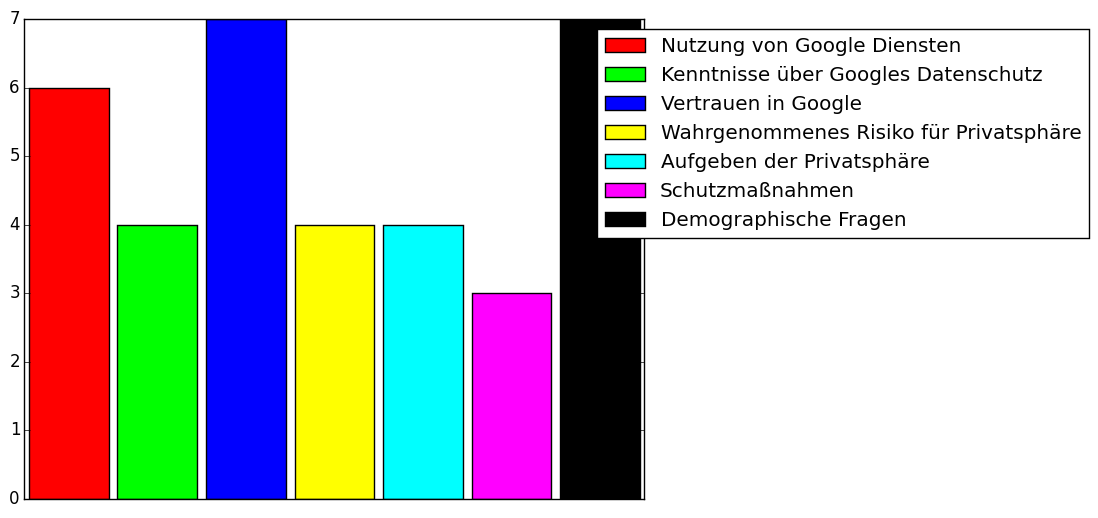
\includegraphics[width=\textwidth]{images/zahlenkategorien}\\
\caption{Anzahl der Fragen pro Kategorie in \ref{sec:categories}}\label{catnumbers}
\end{figure}

\begin{figure}[H]
\centering
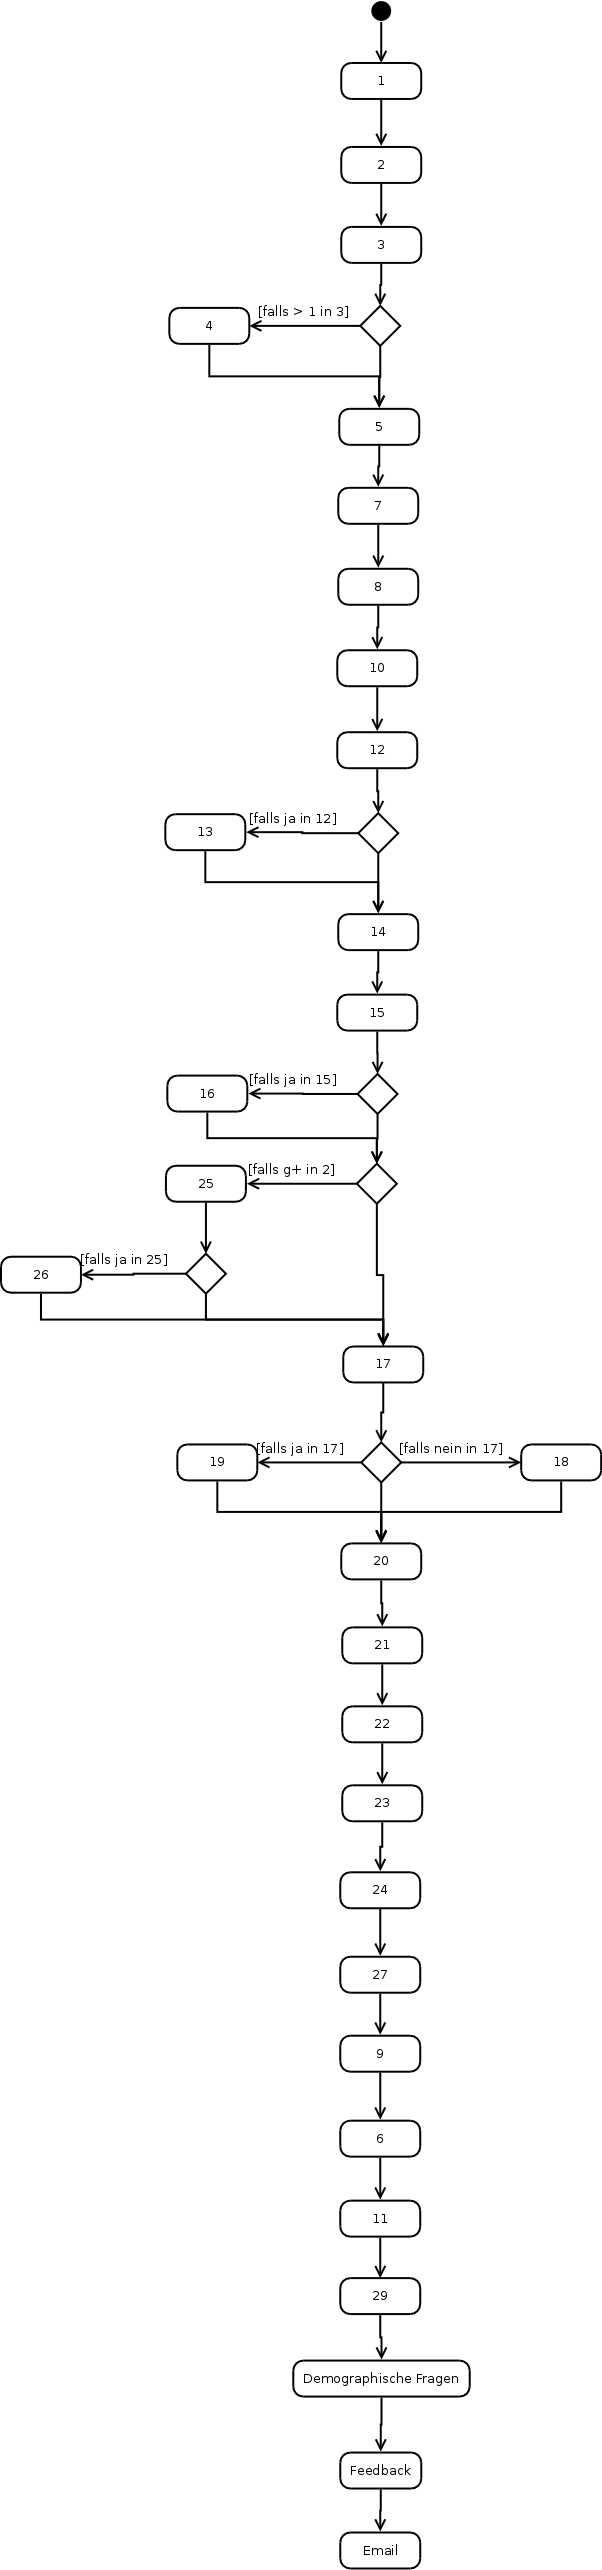
\includegraphics[height=\textheight]{images/umldia}\\
\caption{Anordnung der Fragen}\label{umldia}
\end{figure}


\section{Rekrutierung der Teilnehmer}
Die Umfrage wurde zuerst über Facebook und per Email über Familienmitglieder und Bekannte verteilt, mit der Angabe sie nach Möglichkeit auch weiter zu verteilen. Nachdem so schon eine relativ große Anzahl an Antworten erhalten wurden, wurde die Umfrage noch über den Email-Verteiler der Technischen Fakultät der Universität Erlangen-Nürnberg verbreitet.